The Janus Tough Adhesive has shown to exhibit high biocompatibility during testing, despite it containing the synthetic polymer polyacrylamide. To evaluate their performance and impact on natural tissues, \citeauthor{freedmanEnhancedTendonHealing2022} (\citeyear{freedmanEnhancedTendonHealing2022}) experimentally tested  injured and healthy rats, and applied the JTA to the patellar tendon.
For three weeks, potential swelling of the tendon and degredation of the gel were assessed by high frequency ultrasound. When a tendon becomes injured, its echogenicity---the amount of sound it reflects---decreases, because its collagen fibres become more disorganised and less densely packed \autocite{hodgsonTendonLigamentImaging2012}.
Researchers also found that injured tendons without application of the JTA had larger cross-section areas, indicating increased swelling as shown in Figure~\ref{fig:JTA_Patellar_cross_section} below. A decrease in inflammation in the affected tendon therefore suggests that the JTA was effective and well-tolerated by the body.
\begin{figure}[h]
    \centering
    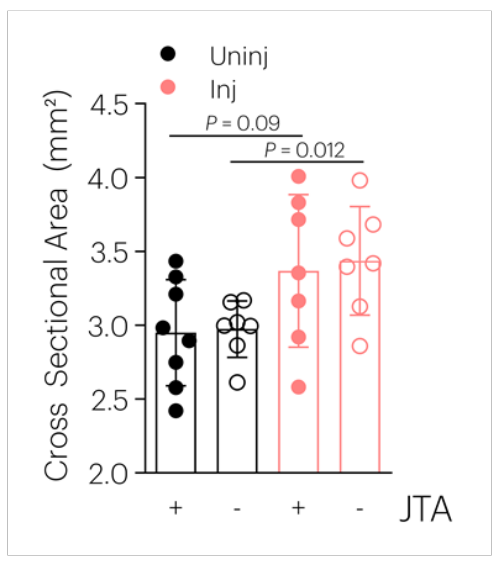
\includegraphics[width=0.6\linewidth]{JTA_cross_section.png}
    \caption{Patellar tendon cross-sectional area (mm\textsuperscript{2}) after 3 weeks of treatment [Adapted from \cite{freedmanEnhancedTendonHealing2022}]}
    \label{fig:JTA_Patellar_cross_section}
\end{figure}

Furthermore, in the patellar tendon, the JTA was found to have improved tendon relaxation (Figure~\ref{fig:JTA_Patellar_relaxation}), without impacting natural properties such as elastic mechanics, dynamic modulus, or linear modulus.
\begin{figure}[h]
    \centering
    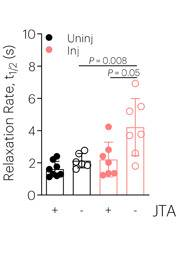
\includegraphics[width=0.6\linewidth]{Figures/JTA_relaxation_patellar.jpeg}
    \caption{Patellar tendon relaxation rate [Adapted from \cite{freedmanEnhancedTendonHealing2022}]}
    \label{fig:JTA_Patellar_relaxation}
\end{figure}

Biocompatibility of the JTA was also tested in more complex use cases, such as the rotator cuff and Achilles tendon. 